\section{Auswertung}

\begin{frame}{Inhaltsverzeichnis}
    \tableofcontents[currentsection, hidesubsections]
\end{frame} 

\subsection{Maße}

\begin{frame}{Auswertung}
    \begin{block}{Maße}
    Masse $m = \SI{435.64}{\gram}$

    Höhe über Boden $l= \SI{26.4}{\centi\meter}$
    
    Radius des Rades $R =\SI{6.35}{\centi\meter}$
    
    Radius des Schwerpunkts zur Mitte(gemessen) $r= \SI{3}{\milli\meter}$
    \end{block}
\end{frame}
\subsection{Gemessener Radius}
\begin{frame}{Auswertung}

    \begin{block}{Gemessener Radius}
        Der Radius ergibt sich zu r= 3.279 \si{\milli\meter}. 
    \end{block}
\end{frame}

\subsection{Plots - lineare Regression}

\begin{frame}{Plots - lineare Regression}
    \begin{figure}   
    
    \centering
    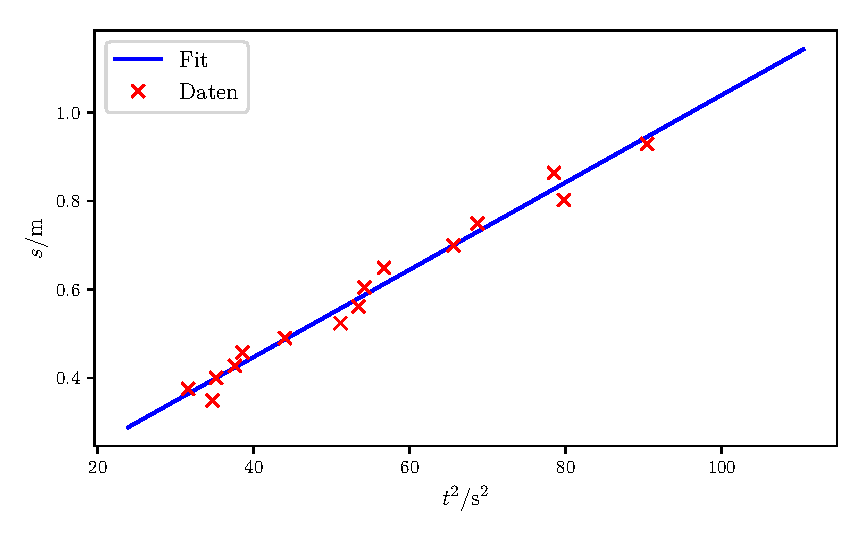
\includegraphics[width=8cm, height=6cm]{build/plot1b.pdf}
    \caption{Ein Graph.} 

    \label{fig:plot1b}
\end{figure}
\end{frame}

\begin{frame}
    \begin{figure}   
    
    \centering
    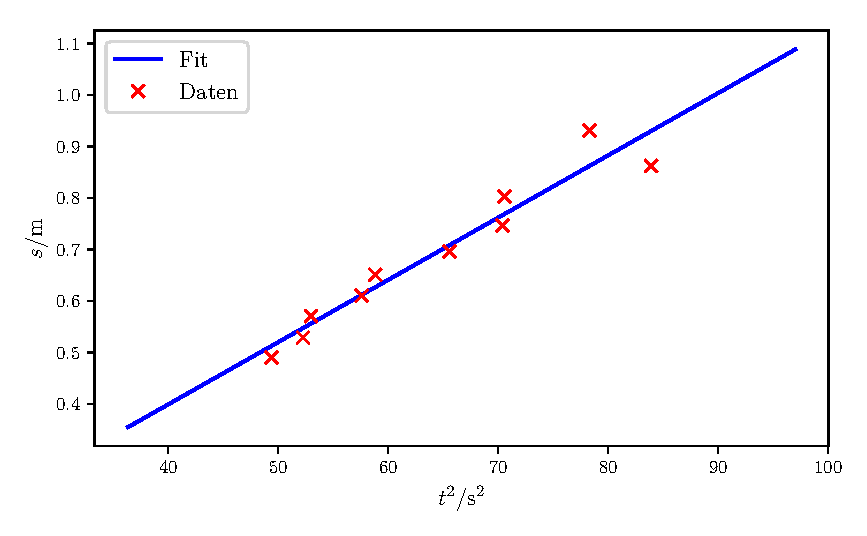
\includegraphics[width=8cm, height=6cm]{build/plot2b.pdf}
    \caption{Ein Graph.} 

    \label{fig:plot2b}
\end{figure}
\end{frame}

\begin{frame}
    \begin{figure}   
    
    \centering
    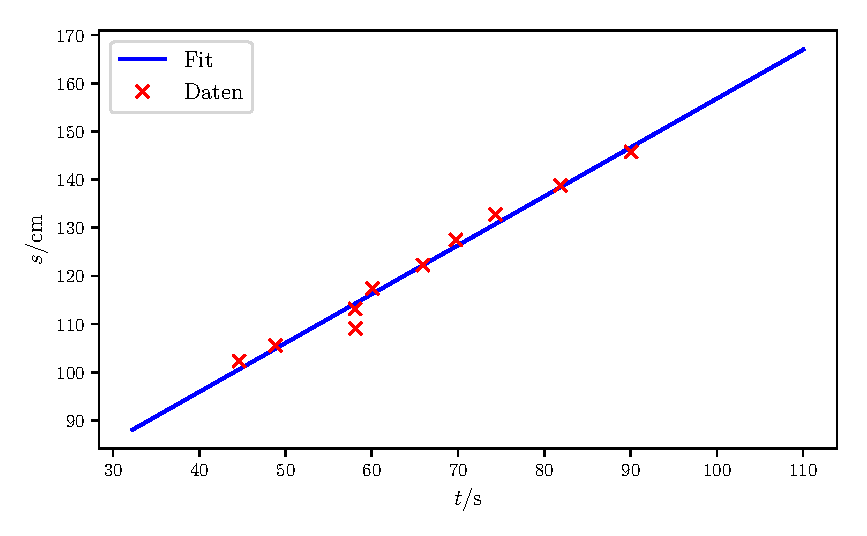
\includegraphics[width=8cm, height=6cm]{build/plot3b.pdf}
    \caption{Ein Graph.} 

    \label{fig:plot3b}
\end{figure}
\end{frame}

\subsection{Beschleunigung}
\begin{frame}
    \begin{block}{Beschleunigung}
        
        Die mittlere Steigung die sich ergibt ist s=0.535 +/- 0.049 \si{\centi\meter\per\second}.
    \end{block}
\end{frame}
    
\subsection{Plots - Tatsächliche Daten}
\begin{frame}
    \begin{figure}   
    
    \centering
    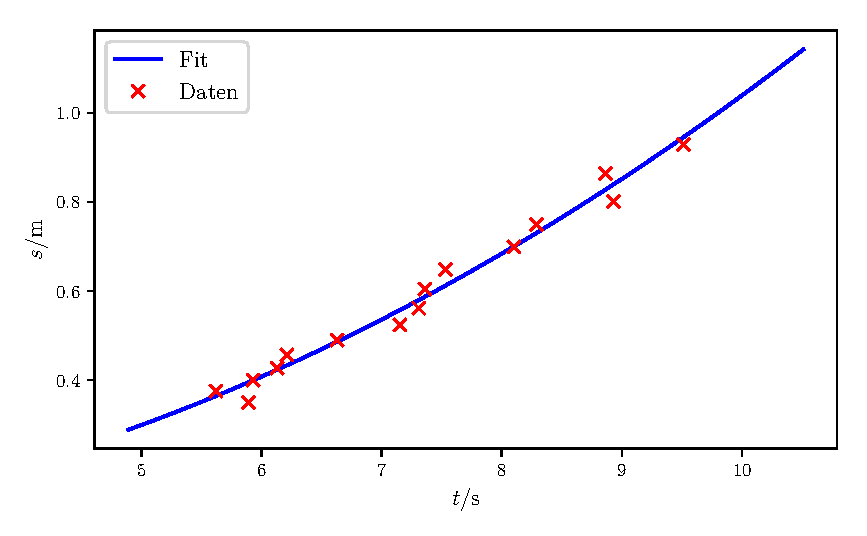
\includegraphics[width=8cm, height=6cm]{build/plot1a.pdf}
    \caption{Ein Graph.} 

    \label{fig:plot1a}
\end{figure}
\end{frame}

\begin{frame}
    \begin{figure}   
    
    \centering
    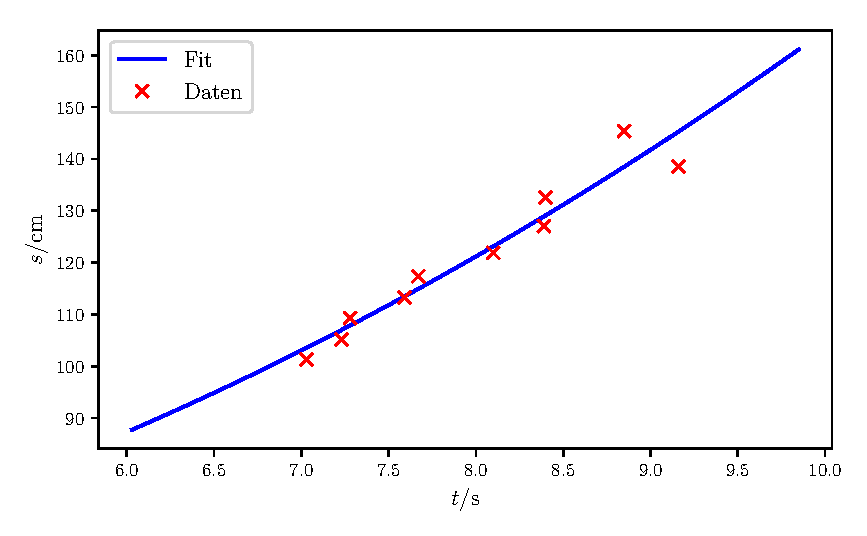
\includegraphics[width=8cm, height=6cm]{build/plot2a.pdf}
    \caption{Ein Graph.} 

    \label{fig:plot2a}
\end{figure}
\end{frame}

\begin{frame}
    \begin{figure}   
    
    \centering
    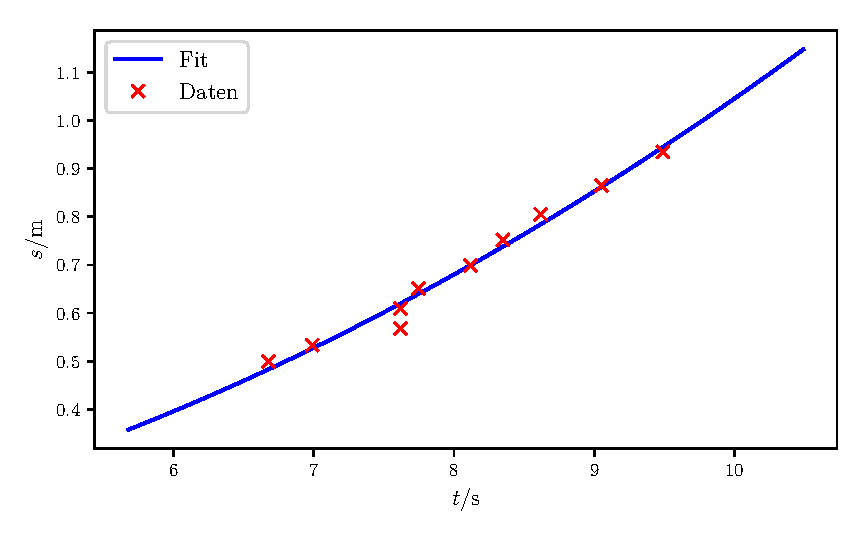
\includegraphics[width=8cm, height=6cm]{build/plot3a.pdf}
    \caption{Ein Graph.} 

    \label{fig:plot3a}
\end{figure}
\end{frame}

\begin{frame}
    \begin{figure}   
    
    \centering
    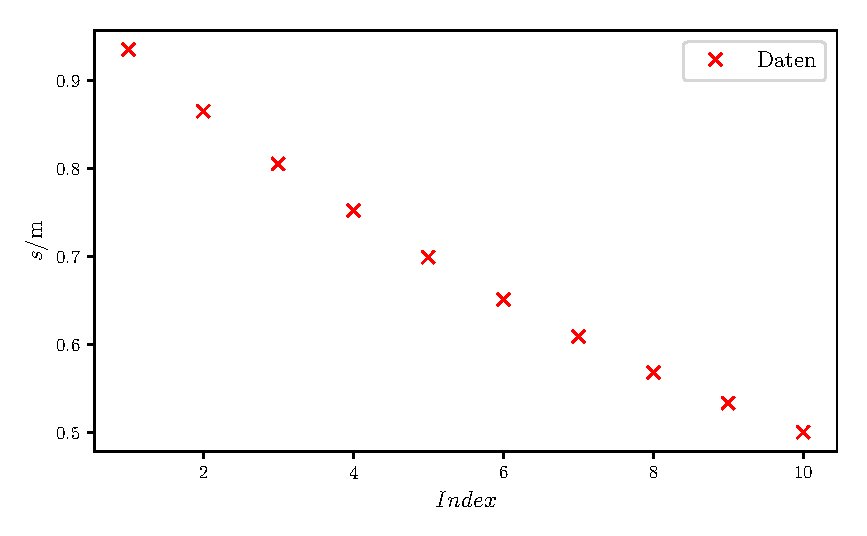
\includegraphics[width=8cm, height=6cm]{build/plot5a.pdf}
    \caption{Ein Graph.} 

    \label{fig:plot5}
\end{figure}
\end{frame}

